\documentclass[pdftex,12pt,a4paper]{article}

% техническая часть
\usepackage{makeidx}
\usepackage{cmap}
\usepackage[pdftex]{graphicx} 
\usepackage[colorlinks,hyperindex,unicode]{hyperref}

\usepackage[utf8]{inputenc}
\usepackage[T2A]{fontenc} 
\usepackage[russian]{babel}

% что будет в заголовке...
\title{Немного обо мне}
\author{Поросёнок Хрюша}
\date{\today}

\begin{document}
\maketitle % размещаем заголовок здесь!

Несколько интересных фактов обо мне:

\begin{enumerate}
\item День рождения --- 10 февраля 1971 года
\item Амплуа --- непослушный ребёнок
\item Участвовал в передаче <<Нержавеечка>> для металхэдов
\item <<Мощно задвинул, внушаить!>>
\item 31 июля 2012 года я организовал одиночный пикет в Екатеринбурге
\end{enumerate}


% можно использовать форматы jpg, png и pdf 
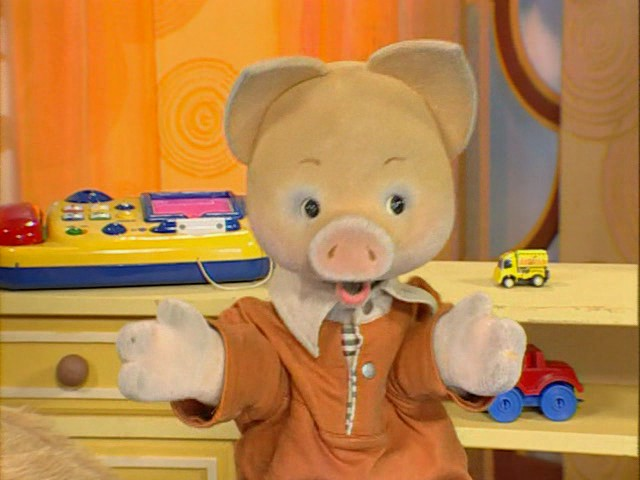
\includegraphics[height=3in]{khrusha.jpg}


\end{document}
